\chapter{Analysis under Terminal Constraints}\label{ch:bridging}
% Observations of the \ac{MPM} are typically based on noisy measurements.
% In most applications, they give only partial information about the
% system state and are sparse in time.
% For example, snapshots of the spread of an epidemic are typically
% not accurate due to false negative/positive results and limited testing.
Many tasks, such as the analysis of rare events or the inference of
agent counts under partial observations naturally introduce terminal
constraints on the system.
In these cases, the system's initial state is known, as well as the
system's (partial) state at a later time-point.
% Parameter inference and model analysis conditioned on such sparse
% and partial observations are notoriously difficult as it requires
% endpoint conditioned simulation of the system.
% Essentially, a model must be  analyzed  with initial conditions
% consistent with the observations at one time-point and under the
% additional constraint that its subsequent evolution is consistent
% with observations at later times.
The probabilities corresponding to this so-called \emph{bridging
problem} are often referred to as \emph{bridging probabilities}
\parencite{golightly2019efficient,golightly2011bayesian}.
For instance, if the exact, full state of the process $X_t$ has been
observed at time $t=0$ and $t=T$, the bridging distribution is given by
\[
  \Pr(X_t=x\mid X_{0}=x_{0},X_{T}=x_g)
\]
for all states $x$ and times $t\in [0,T]$.
Often, the condition is more complex, such that in addition to an
initial distribution, a terminal distribution is present.
Such problems typically arise in a Bayesian setting, where the a
priori behavior of a system is filtered such that the posterior
behavior is compatible with noisy, partial
observations~\parencite{broemeling2017bayesian,huang2016reconstructing}.
For example, time-series data of protein levels is available while
the \acsfont{mRNA} concentration is not
\parencite{adan2017flow,huang2016reconstructing}.
In such a scenario our method can be used to identify a good
truncation to analyze the probabilities of \acsfont{mRNA} levels.
% Such measurements are, for example, present in biological
% flow-cytometry \parencite{adan2017flow} data.
% This technique allows one to measure protein concentrations at
% specific time points based on fluorescent labeling.
% Such measurements are noisy due to low signal intensity and can,
% for instance, not measure whether a gene is active or not.
% A similar problem
% \todo{finish sentence}

% In \acp{HMM}  the backward-forward algorithm
% decomposes the bridging problem into a forward and a backward
% analysis to calculate the marginal likelihood and calibrate the
% model according to noisy observations. \vw{haben wir da ein Zitat
% mit population structure und contin.-time? Hier das ist eigentlich
% eine HMM \parencite{andreychenko2012approximate} }\todo{Luca:
% nicely written, but what is the link with our framework?}

Bridging probabilities also appear in the context
of rare events.
Here, the rare event is the terminal constraint because we are only
interested in paths containing the event.
Typically researchers have to resort to Monte Carlo simulations in
combination with variance reduction techniques in such
cases~\parencite{daigle2011automated,kuwahara2008efficient}.
% For instance, we may want to
% compute the probability of the rare event that the number of
% molecules of a certain chemical species reaches a certain cellular
% decision threshold \parencite{daigle2011automated,kuwahara2008efficient}.

Efficient  numerical approaches  that are not based on sampling or
ad-hoc approximations have rarely been developed.

Here, we combine state-of-the-art truncation strategies based on a
forward analysis~\parencite{lapin2011shave,andreychenko2011parameter}
with a refinement approach that starts from an abstract \ac{MPM}
with lumped states.
We base this lumping on a grid-like partitioning of the state-space.
Throughout a lumped state, we assume a uniform distribution that
gives an efficient and convenient abstraction of the original \ac{MPM}.
Note that the lumping does not follow the classical paradigm of
Markov chain lumpability~\parencite{buchholz1994exact}
or its variants \parencite{dayar1997quasi}.
Instead of an approximate block structure of the transition-matrix
used in that context, we base our partitioning on a segmentation of
the molecule counts.
Moreover, during the iterative refinement of our
abstraction, we identify those regions of
the state-space that contribute most to the
bridging distribution.
In particular, we refine those lumped states that have a
bridging probability above a certain threshold $\delta$ and
truncate all other macro-states.
This way, the algorithm learns a truncation capturing most of the
bridging probabilities.
This truncation provides guaranteed lower bounds because it is at the
granularity of the original model.

\section{Related Work}\label{sec:bridging:related}
\paragraph{Terminal Constraints}
The problem of endpoint constrain\-ed analysis occurs in the context
of Bayesian estimation~\parencite{sarkka2013bayesian}.
For \acp{MPM}, this problem has been addressed by
\citet{huang2016reconstructing} using moment closure approximations
and by \citet{wildner2019moment} further employing variational inference.
Golightly and Sherlock modified stochastic simulation algorithms to
approximatively
augment generated trajectories  \parencite{golightly2019efficient}.
% The idea is to  sample trajectories that are consistent with
% measurements, which requires sampling   appropriate values for
% latent state variables and sampling appropriate events between two
% observation times.
Since a statistically exact augmentation is only possible for few
simple cases, diffusion approximations
\parencite{golightly2005bayesian} and moment approximations
\parencite{milner2013moment} have been employed.
Such approximations, however, do not give any guarantees on the
approximation error
and may suffer from numerical instabilities~\parencite{schnoerr2014validity}.

Another manifestation of the bridging problem is found during the
estimation of first passage times and rare event analysis.
Approaches for first-passage times are often of heuristic nature
~\parencite{schnoerr2017efficient,hayden2012fluid,bortolussi2014stochastic}.
Rigorous approaches yielding guaranteed bounds are currently limited
by the performance of state-of-the-art optimization
software~\parencite{backenkohler2019bounding}.

\paragraph{Rare Event Probabilities}
The analysis of rare events is a special case of the terminal
constrained Markov processes considered in this chapter.
Most methods for the estimation of rare event probabilities  rely on
importance sampling~\parencite{kuwahara2008efficient,daigle2011automated}.
For other queries, alternative variance reduction techniques such as
control variates are available~\parencite{backenkohler2019control}.
Apart from sampling-based approaches, dynamic finite-state
projections have been employed by \citet{mikeev2013numerical}, but
are lacking automated truncation schemes.

\paragraph{State-Space Truncation}
The analysis of countably infinite state-spaces is often handled by a
pre-defined truncation~\parencite{kwiatkowska2011prism}.
Sophisticated state-space truncations for the (unconditioned) forward
analysis have been developed to give lower bounds and rely on a
trade-off between computational load and tightness of the
bound~\parencite{munsky2006finite,lapin2011shave,andreychenko2011parameter,henzinger2009sliding,mikeev2013fly}.

\paragraph{Verification}
The problem considered in this chapter can be interpreted as an
instance of a model checking problem \parencite{brim2013model,BENTRIOU2021191}.
Reachability --~relevant in the context of probabilistic verification
\parencite{bortolussi2014stochastic,neupane2019stamina}~-- is a
bridging problem where the endpoint constraint is the visit of a set
of goal states.
Backward probabilities are commonly used to compute reachability
likelihoods \parencite{amparore2013backward,zapreev2006safe}.
Approximate techniques for reachability, based on moment closure and
stochastic approximation, have also been developed in
\parencite{bortolussi2014stochastic,Bortolussi18infcomp}, but lack
error guarantees.

\paragraph{Hidden Markov Models}
There is also a conceptual similarity between computing bridging
probabilities and the forward-backward algorithm for computing
state-wise posterior marginals in
\acfp{HMM}~\parencite{rabiner1986introduction}. Like \acp{MPM},
\acp{HMM} are a generative model that can be conditioned on
observations. We only consider two observations (initial and terminal
state) that are not necessarily noisy but the forward and backward
probabilities admit the same meaning.

\section{Backward Probabilities}
Let $x_g\in \mathcal{S}$ be a fixed goal state.
Given the terminal constraint
\begin{equation*}
  \Pr(X_T=x_g)=1 \text{ for some }T\geq 0\,,
\end{equation*}
we are interested in the so-called backward probabilities
\begin{equation}\label{eq:back_probs}
  \beta(x_i, t) = \Pr(X_T=x_g\mid X_t = x_i),\quad t\leq T\,.
\end{equation}
Note that $\beta(\cdot, t)$ is a function of the conditional event
and thus is no probability distribution over the state-space.
Instead $\beta(\cdot, t)$ gives the reaching probabilities for all
states over the
time span of $[t, T]$.
To compute these probabilities, we can employ the Kolmogorov backward equation
\begin{equation}\label{eq:backward}
  \frac{d}{dt}\beta(t) = Q\beta(t)\,,
\end{equation}
where we use the same vectorization to construct $\beta(t)$ as we used
for $\pi(t)$.
The above equation is integrated backwards in time and yields the reachability
probability for each state $x_i$ and time $t<T$ of ending up in $x_g$
at time $T$.
Similar to the \ac{CME} \eqref{eq:cme}, we can state a backward
chemical master equation
\begin{equation}\label{eq:bcme}
  \frac{d\beta}{dt}({x}, t) =
  \sum_{j=1}^{n_R}\left(
    \beta( x,t) - \beta( x+ v_j,t)
  \right)\alpha_j({x})\,.
\end{equation}

The state-space of many \acp{MPM}, even simple ones, is countably infinite.
In this case, we have to truncate the state-space to a \emph{reasonable}
finite subset.
The choice of this truncation heavily depends on the goal of the
analysis.
If one is interested in the most ``common'' behavior, for example,
a dynamic mass-based truncation scheme is most appropriate
\parencite{mikeev2019approximate}.
Such a scheme truncates states with small probability during the
numerical integration.
However, common mass-based truncation schemes are not as useful for the
bridging problem. This is because trajectories that meet
the specific terminal constraints can be far off the main bulk of the
probability mass.
We solve this problem by a state-space lumping in connection with an
iterative refinement scheme.

\section{Bridging Distribution}\label{sec:bridge_dist}
The process' probability distribution given both initial and terminal
constraints is formally described  by
the conditional probabilities
\begin{equation}\label{eq:bridge_dist}
  \gamma(x_i, t) = \Pr(X_t = x_i \mid X_0 = x_0, X_T = x_g)\,,
\end{equation}
for $0\leq t\leq T$.
for fixed initial state $x_0$ and terminal state $x_g$.
We call these probabilities the \emph{bridging probabilities}.
It is straight-forward to see that      $\gamma$ admits the
factorization
\begin{equation}\label{eq:bridge_fact}
  \gamma(x_i, t) = \pi(x_i, t)\beta(x_i, t)/\pi(x_g, T)
\end{equation}
due to the Markov property.
The normalization factor, given by the reachability probability
\[
  \pi(x_g, T)=\beta(x_0, 0)\,,
\]
ensures that $\gamma(\cdot, t)$ is
a distribution for all time points $t\in[0,T]$.
We call each $\gamma(\cdot, t)$ a   \emph{bridging distribution}.
From the Kolmogorov equations \eqref{eq:forward}\turnto{eq:forward}
and \eqref{eq:backward}
we can obtain both the forward probabilities $\pi(\cdot, t)$ and the
backward probabilities
$\beta(\cdot, t)$ for $t< T$.

We can easily extend this procedure to deal with hitting times
constrained by a finite time-horizon by making the goal state $x_g$ absorbing.

\begin{example}
  In \autoref{fig:bd_bridge} we plot the forward, backward, and
  bridging probabilities for \autoref{model:bd}\turnto{model:bd}.
  The probabilities are computed on a $[0,100]$ state-space truncation.
  The approximate forward solution $\hat\pi$ shows how the
  probability mass drifts upwards towards the stationary distribution
  $\text{Poisson}(100)$. The backward probabilities are highest for
  states below the goal state $x_g=40$.
  This is expected because upwards drift makes reaching $x_g$ more
  probable for ``lower'' states.
  Finally, the approximate bridging distribution $\hat\gamma$ can be
  recognized to be proportional to the product of forward $\hat\pi$
  and backward probabilities $\hat\beta$.
  \begin{figure}[htb]
    \centering
    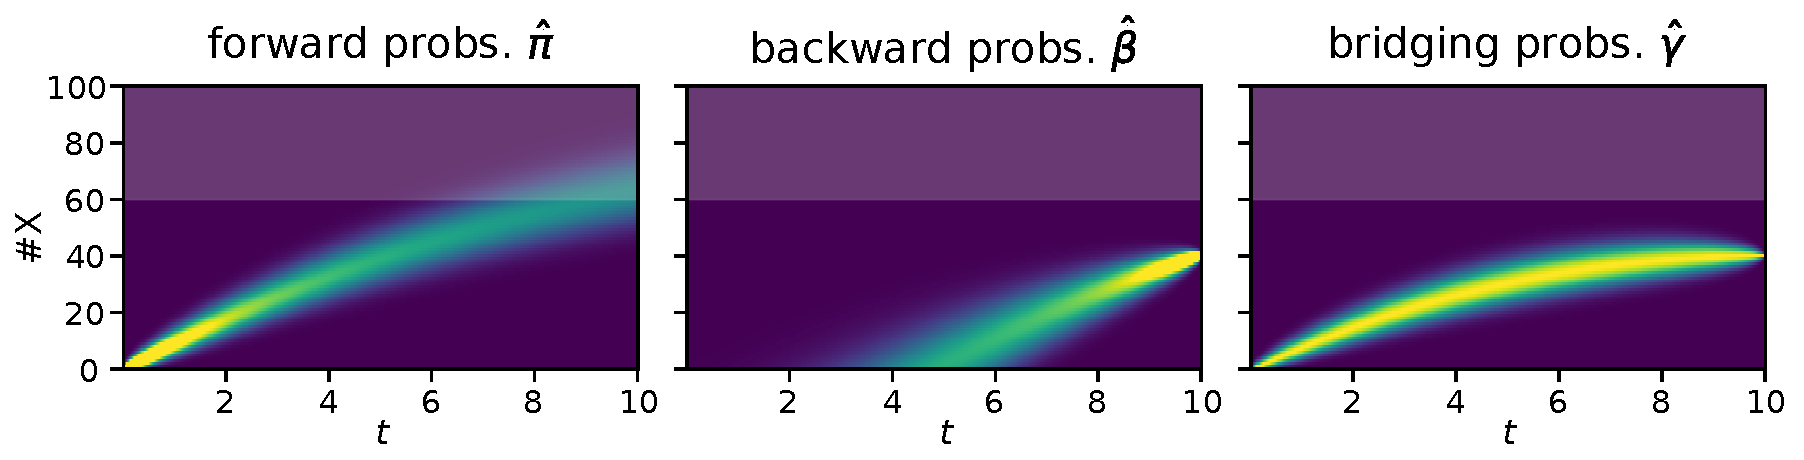
\includegraphics[width=\textwidth]{gfx/bridging_bd.pdf}
    \caption[Forward, backward, and bridging probabilities for
    \autoref{model:bd}]{Forward, backward, and bridging probabilities
      for \autoref{model:bd} with initial constraint $X_0=0$ and
      terminal constraint $X_{10}=40$ on a truncated state-space.
      Probabilities over $0.1$ in $\hat\pi$ and $\hat\beta$ are given
      full intensity for visual clarity. %$\hat\gamma$ is normalized
      % using the reaching probability.
      The lightly shaded area ($\geq 60$) indicates a region being more
    relevant for the forward than for the bridging probabilities.}
    \label{fig:bd_bridge}
  \end{figure}
\end{example}

\section{Bridge Truncation via Lumping Approximation}\label{sec:bridging:method}
We first discuss the truncation of countably infinite state-spaces
to analyze backward and forward probabilities (\autoref{sec:bridging:fsp}).
To identify effective truncations we employ a lumping scheme.
Finally, in \autoref{sec:bridging:alg} we present an iterative
refinement algorithm
yielding a suitable truncation for the bridging problem.

\subsection{Finite State Projection}\label{sec:bridging:fsp}
Even in simple models such as a birth-death Process (\autoref{model:bd}), the
reachable state-space is countably infinite.
Direct analyzes of backward \eqref{eq:back_probs} and forward
equations \eqref{eq:forw_prob}\turnto{eq:forw_prob} are often infeasible.
Instead, the integration of these differential equations requires working
with a finite subset of the infinite state-space \parencite{munsky2006finite}.
If states are truncated, their incoming transitions from states that
are not truncated can be re-directed to a \emph{sink state}.
The  accumulated probability in this sink state is then used
as an error estimate for the forward integration scheme.
Consequently, many truncation schemes, such as dynamic truncations
\parencite{andreychenko2011parameter}, aim to minimize the
amount of ``lost mass'' of the forward probability.
We use the same truncation method but base the truncation on bridging
probabilities rather than the forward probabilities.
% We redirect incoming transitions of truncated states to the sink state.
% For all truncated states, we capture the
% corresponding incoming probability mass in a single sink state.

\subsection{Iterative Refinement Algorithm}\label{sec:bridging:alg}
The iterative refinement algorithm (\autoref{alg:refinement}) starts
with a set of large macro-states
that are iteratively refined, based on approximate solutions
to the bridging problem.
We start by constructing square macro-states of size
$2^m$ in each dimension for some $m\in\mathbb{N}$ such that they form
a large-scale grid $\mathcal{S}^{(0)}$.
Hence, each initial macro-state has a volume of ${\left(2^m\right)}^{n_S}$.
This choice of grid size is convenient because we can halve states
in each dimension.
Moreover, this choice ensures that all states have equal volume
and we end up with states of volume $2^0=1$ which is
equivalent to a truncation of the original non-lumped state-space.

An iteration of the state-space refinement starts by computing both the
forward and backward probabilities (\autoref{line:forw} and
\autoref{line:backw})  via integration of
\eqref{eq:forward}\turnto{eq:forward} and
\eqref{eq:backward}, respectively, using
the lumped $\hat Q$-matrix.
Based on the resulting approximate forward and backward probabilities, we
compute an approximation of the
bridging distributions (\autoref{line:bridge}).
This is done for each time-point in an equispaced grid on $[0,T]$.
The time grid granularity is a hyper-parameter of the algorithm.
If the grid is too fine, the memory overhead of storing backward
$\hat\beta^{(i)}$
and forward solutions $\hat\pi^{(i)}$ increases.
{We denote the approximations with a hat (e.g.\ $\hat{\pi}$) rather
  than a bar (e.g.\ $\bar{\pi}$) to indicate that not only the lumping
  approximation but also a truncation is applied and similarly for the
$Q$-matrix.}
If, on the other hand, the granularity is too low, too much of
the state-space might be truncated.
Based on a threshold parameter $\delta>0$
states are either removed or split (\autoref{line:refine}), depending on
the mass assigned to them by the approximate bridging
probabilities $\hat\gamma^{(i)}_t$.
A state can be split by the \texttt{split}-function which
halves the state in each dimension.
Otherwise, it is removed.
Thus, each macro-state is either split into $2^{n_S}$ new states or removed
entirely.
The result forms the next lumped state-space $\mathcal{S}^{(i)}$.
The   $Q$-matrix is adjusted (\autoref{line:update_q}) such that
transition rates  for $\mathcal{S}^{(i)}$  are calculated according to
\eqref{eq:lumped_q}.
Entries of truncated states are removed from the transition matrix.
Transitions leading to them are
re-directed to a sink state (\autoref{sec:bridging:fsp}).
After $m$ iterations (we started with states of side lengths $2^m$)
we have a standard \ac{FSP} scheme
on the original model tailored to
computing an approximation of the bridging distribution.
\begin{algorithm}[htb]
  \SetKwFunction{Split}{split}
  \SetKwInOut{Input}{input}
  \SetKwInOut{Output}{output}
  \Input{initial partitioning $\mathcal{S}^{(0)}$, truncation
  threshold $\delta$}
  \Output{approximate bridging distribution $\hat\gamma$}
  \For{$i=1,\dots,m$}{
    ${\hat\pi}^{(i-1)}_t\leftarrow $ approximate forward equation on
    $\mathcal{S}^{(i)}$\label{line:forw}\;
    ${\hat\beta}^{(i-1)}_t\leftarrow $ approximate backward equation
    on $\mathcal{S}^{(i)}$\label{line:backw}\;
    ${\hat\gamma}^{(i)}_t\leftarrow {\hat\beta}^{(i)}
    {\hat\pi}^{(i)}/\hat\pi(x_g,  T)$\label{line:bridge}\tcc*{approx. bridging}
    $\mathcal{S}^{(i)}\leftarrow \emptyset$\;
    \ForEach{$\bar{x}\in\mathcal{S}^{(i)}$}{
      \If{
        $\exists t.{\hat\gamma}^{(i)}_t(\bar{x})\geq
        \delta$\label{line:refine}\tcc*{refinement}
      }{
        $\mathcal{S}^{(i)}\leftarrow \mathcal{S}^{(i)} \cup
        \Split(\bar{x})$\label{line:union}\;
    }}
    update $\hat{Q}$-matrix\label{line:update_q}\;
  }
  \Return ${\hat\gamma}^{(i)}$\;
  \caption{Iterative refinement for the bridging problem}
  \label{alg:refinement}
\end{algorithm}

In \autoref{fig:refinement} we give a demonstration of how
\autoref{alg:refinement} works to refine the state-space
iteratively. Starting with an initial lumped state-space
$\mathcal{S}^{(0)}$ covering a large area of the state-space,
repeated evaluations of the bridging distributions are performed.
After five iterations the remaining truncation includes all states
that significantly contribute to the bridging
probabilities over the times $[0,T]$.
\begin{figure}[tb]
  \centering
  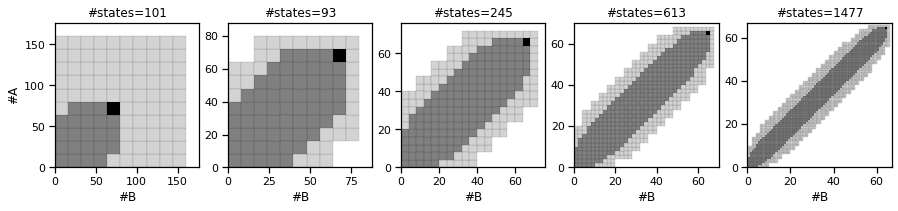
\includegraphics[width=\textwidth]{gfx/refinement.png}
  \caption[State-space refinement algorithm on two parallel unit-rate
  arrival processes]{The state-space refinement algorithm on two
    parallel unit-rate arrival processes. The bridging problem from
    $(0,0)$ to $(64, 64)$ and $T=10$ and truncation threshold
    $\delta=\e{5}{-3}$. States with a bridging probability below
    $\delta$ are light grey. The macro-state containing the goal state
  is marked in black. The initial macro-states are of size $16\times 16$.}
  \label{fig:refinement}
\end{figure}

% das ist nicht spezifisch für rare events. es kann genauso gut sein
% dass bei einem rare event die hauptmasse der forward in der truncation bleibt.
It is important to realize that determining the most relevant states
is \emph{the} main challenge.
The above algorithm solves this problem by considering only those
parts of the state-space that contribute most to the bridging probabilities.
The truncation is tailored to this condition and might ignore regions
that are likely in the unconditioned case.
For instance, in \autoref{fig:bd_bridge} the bridging probabilities
mostly remain below a population threshold of $\#X=60$ (as indicated
by the lighter/darker coloring), while the forward probabilities
mostly exceed this bound. Hence, in this example a significant
portion of the forward probabilities $\hat\pi_t^{(i)}$
is captured by the sink state. However, the condition in
\autoref{line:refine} of \autoref{alg:refinement} ensures that
states contributing significantly to $\hat\gamma_t^{(i)}$ will be
kept and refined in the next iteration.


\section{Results}\label{sec:bridging:results}
We present four examples in this section to evaluate our proposed method.
A prototype was implemented in Python~3.8. For numerical integration
we used the Scipy implementation \parencite{2020SciPy-NMeth} of the
implicit method based on backward-differentiation formulas
\parencite{byrne1975polyalgorithm}.
The analysis as a Jupyter notebook is made available
online~\parencite{mjp_bridging}.

\subsection{Bounding Rare Event Probabilities}
We consider a simple model of two parallel Poisson processes
describing the production of two
types of agents.
The corresponding probability distribution
has Poisson product form at all time points $t\geq 0$ and hence we
can compare the accuracy of our  numerical results with the exact
analytic solution.
We use the proposed approach to compute lower bounds for rare event
probabilities.
These bounds are rigorous up to the approximation error of the
numerical integration scheme.
However, the forward solution could be replaced by an
uniformization\turnto{item:uniformization} approach for a more
rigorous error control.

\begin{model}[Parallel Poisson Processes]\label{model:par_poisson}
  The model consists of two parallel independent Poisson processes
  with unit rates.
  $$ \varnothing \xrightarrow{1} A \qquad\text{and}\qquad \varnothing
  \xrightarrow{1} B\,. $$
  The initial condition $X_0=(0,0)$ holds with probability one. After
  $t$ time units each species abundance
  is Poisson distributed with rate $\lambda=t$.
\end{model}
We consider the final constraint of reaching a state where both
processes exceed a threshold of $64$ at time $20$.
Without prior knowledge, a reasonable truncation would have been
$160\times 160$. But our analysis shows that just \num{20}\% of the
states are necessary to capture over \num{99.6}\% of the probability
mass reaching the
target event (cf.\ \autoref{tab:par_poisson}).
Decreasing the threshold $\delta$ leads to a larger set of states
retained after truncation as more of the bridging distribution is
included (cf.\ \autoref{fig:2poisson_rare}).
We observe an increase in truncation size that is approximately
logarithmic in $\delta$, which, in this example, indicates robustness
of the method with respect to the choice of $\delta$.
\begin{figure}[!t]
  \centering
  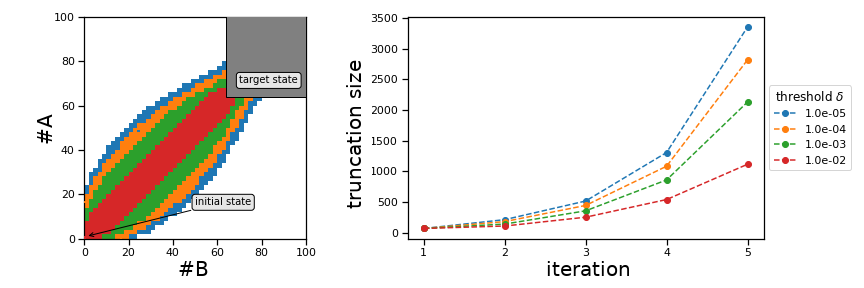
\includegraphics[width=\textwidth]{gfx/truncs.png}
  \caption[State-space truncation for varying values of the
  threshold parameter $\delta$]{State-space truncation for varying values of the
    threshold parameter $\delta$: Two parallel Poisson processes
    under terminal constraints $X_{20}^{(A)} \geq 64$ and $X_{20}^{(B)}\geq 64$.
    The initial macro-states are $16\times 16$ such that the final
  states are regular micro states.}
  \label{fig:2poisson_rare}
\end{figure}

%\setlength{\tabcolsep}{10pt}
\begin{table}[!t]
  \centering
  {\small
    \begin{tabular}{lrrrr}
      \toprule
      & \multicolumn{4}{c}{threshold $\delta$}\\ \cmidrule(lr){2-5}
      & \e{1}{-2} & \e{1}{-3} & \e{1}{-4} & \e{1}{-5} \\
      \midrule
      $|\mathcal{S}^{(m)}|$ & $1154$ & $2354$ & $3170$ & $3898$ \\
      $\sum_m|\mathcal{S}^{(m)}|$\hspace{-1ex} & $2074$ & $3546$ &
      $4586$ & $5450$ \\
      estimate& \e{8.88}{-30} & \e{1.85}{-29} & \e{1.86}{-29} & \e{1.86}{-29} \\
      rel.\ error& \e{5.22}{-1} & \e{3.66}{-3} & \e{3.74}{-5} & \e{9.52}{-8} \\
      \bottomrule
  \end{tabular}}
  \caption[Rare event analysis on the \autoref{model:bd}]{Estimated
    reachability probabilities based on varying truncation thresholds
    $\delta$: The true probability is
    \e{1.8625}{-29}. We also report the size of the final truncation
    $|\mathcal{S}^{(m)}|$ and the accumulated size of all truncations
  during refinement iterations (overall states) $\sum_m|\mathcal{S}^{(m)}|$.}
  \label{tab:par_poisson}
\end{table}

\paragraph{Comparison to other methods}
The truncation approach that we apply  is similar  to the one used by
\citet{mikeev2013numerical} for rare event estimation.
However,  they used a given linearly biased \ac{MPM} model to obtain
a truncation. A general strategy to compute an appropriate biasing
was not proposed.
It is possible to adapt our truncation approach to the dynamic scheme
in \citet{mikeev2013numerical} where states are removed in an
on-the-fly fashion during numerical integration.
% For this dynamic adaption one can change the union over all time points
% (\autoref{alg:refinement} \autoref{line:union}) to a union
% over time intervals. \todo{L: I do not get this really? line 7 is
% the split. } % MB: this point is not important

A finite state-space truncation covering the same area as the initial
lumping approximation would contain $25,\!600$ states.\graffito{The
  goal  is not treated as a single state. Otherwise, it consisted of
$24,\!130$ states.}
The standard approach would be to build up the entire state-space for
such a model \parencite{kwiatkowska2011prism}.
Even using a conservative truncation threshold $\delta=\e{1}{-5}$,
our method yields an accurate estimate using only about a fifth
(\num{5450}) of this accumulated over all intermediate lumped approximations.
% Moreover the analysis yields intermediate distributions which we
% would not obtain using PRISM.

\subsection{Mode Switching}
%Next, we turn to ``mode switching'' events.
%These occur in models exhibiting a \emph{multi-modal} behavior,
% which are of great relevance in
%many contexts~\parencite{siegal2011emergence}. These models exhibit
% a multi-modal stationary distribution.
Mode switching occurs in models exhibiting   \emph{multi-modal} behavior
%(see \autoref{sec:multimodality} for details)
when a trajectory   traverses a potential barrier from one mode
to another.
\graffito{This often is an instance
of rare-event analysis.}
Often, mode switching is a rare event and occurs in the context of
gene regulatory networks where a mode is characterized by the set of
genes being currently active~\parencite{loinger2007stochastic}.
Similar dynamics also commonly occur in queuing models where a system
may for example switch its operating  behavior stochastically if
traffic increases above or decreases below certain thresholds.
Using the presented method, we can get both a   qualitative and
quantitative understanding of   switching
behavior without resorting to Monte-Carlo methods such as   importance sampling.
% In the most common importance sampling scheme, for example,
% rate functions are biased using linear constants, fitted according
% to a cross-entropy objective~\parencite{daigle2011automated}.
% These biased paths are not necessarily representative of the bridging
% distributions.
%Thus we can gain a deeper insight into
%the actual mechanics of mode switching.
% \begin{itemize}
%     \item Mode Switching as a subclass of rare event problems
%     \item Switching dynamics are of biological interest (cell cycle
% control, stuff like that)
%     \item Very common ``sub-module'' of more complex models
%     \item Especially hard to tackle for standard FSP methods
% (multi-modal stationary distribution)
% \end{itemize}

\subsubsection*{Exclusive Switch}
The exclusive switch~\parencite{barzel2008calculation}  has three
different modes of operation, depending on the
\acsfont{DNA} state, i.e.\ on whether a protein of type one or two is bound to
the \acsfont{DNA}.

\begin{model}[Exclusive Switch]\label{model:excl_switch_2} The
  exclusive switch model consists of a promoter region
  that can express both proteins $P_1$ and $P_2$. Both can bind to
  the region, suppressing
  the expression of the other protein. For certain parameterizations,
  this leads to a
  bi-modal or even tri-modal behavior.
  \begin{gather*}
    D + P_1 \xrightarrow{\beta} D.P_1\,,\quad
    D.P1 \xrightarrow{\gamma_1} D + P_1  \,,\\
    D + P_2 \xrightarrow{\beta} D.P_2 \,,\quad
    D.P2 \xrightarrow{\gamma_2} D + P_2 \,,\\
    D.P_1 \xrightarrow{\rho_1} D.P_1 + P_1\,, \quad
    D.P_2 \xrightarrow{\rho_2} D.P_2 + P_2\,,\\
    D \xrightarrow{\rho_1} D + P_1\,,\quad
    D \xrightarrow{\rho_2} D + P_2\,,  \quad
    P_1 \xrightarrow{\lambda}\varnothing  \,,\quad
    P_2\xrightarrow{\lambda} \varnothing
  \end{gather*}
  The parameter values are $\rho=\e{1}{-1}$, $\lambda=\e{1}{-3}$,
  $\beta=\e{1}{-2}$, and $\gamma=\e{8}{-3}$.
\end{model}
Since we know a priori of the three distinct operating modes, we adjust
the method slightly:
The state-space for the \acsfont{DNA} states is not lumped. Instead we ``stack''
lumped approximations of the $P_1$-$P_2$ phase space upon each other.
Special treatment of \acsfont{DNA} states is common for such models
\parencite{lapin2011shave}.

%We assess the switching dynamics from one mode to another.
To analyze the switching, we choose the transition
from\graffito{Variable order: $P_1$, $P_2$, $D$, $D.P_1$, $D.P_2$.}
\[
  x_{1} = (32, 0, 0, 0, 1)
  \quad
  \text{to}
  \quad
  x_2 = (0, 32, 0, 1, 0)
\]
over the time interval $t\in[0,10]$.
The initial lumping scheme covers up to \num{80} molecules of $P_1$
and $P_2$ for each mode.
Macro-states have size $8\times8$ and
the truncation threshold is $\delta=\e{1}{-4}$.

In the analysis of biological switches, not only the switching probability
%is of interest to the researcher.
%The
but also the switching dynamics is a central part of understanding
the underlying biological mechanisms.
In \autoref{fig:switching_dynamics:modes}, we therefore plot the
time-varying probabilities of the gene state conditioned on the mode.
We observe a rapid unbinding of $P_2$, followed by a slow increase of
the binding probability for $P_1$.
These dynamics are already qualitatively captured by the first lumped
approximation (dashed lines).
% \begin{itemize}
%     \item emphasize that we not only get rare event
% prob.\ estimates but insights on the dynamics leading there
%     \item explain how mode switching dynamics
%     \item Compare/contrast coarse- and fine-grained
% \end{itemize}
\begin{figure}
  \centering
  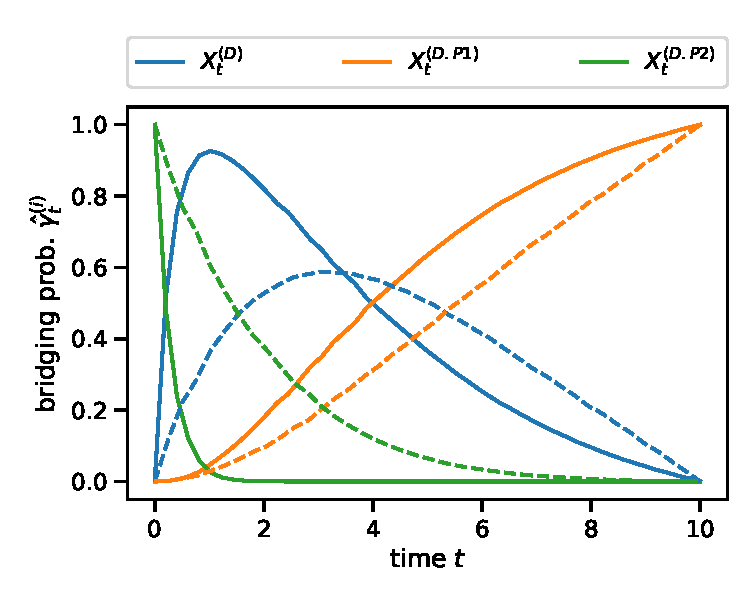
\includegraphics[scale=.6]{gfx/excl_switch_modeprobs.pdf}
  \caption[Mode probabilities of the exclusive switch bridging
  problem]{Mode probabilities of the exclusive switch bridging
    problem over time for the first lumped approximation (dashed lines)
    and the final approximation (solid lines) with constraints
    $X_0=(32, 0, 0, 1, 0)$ and $X_{10}=(0,32,0,0,1)$.
  \label{fig:switching_dynamics:modes}}
\end{figure}
\begin{figure}
  \centering
  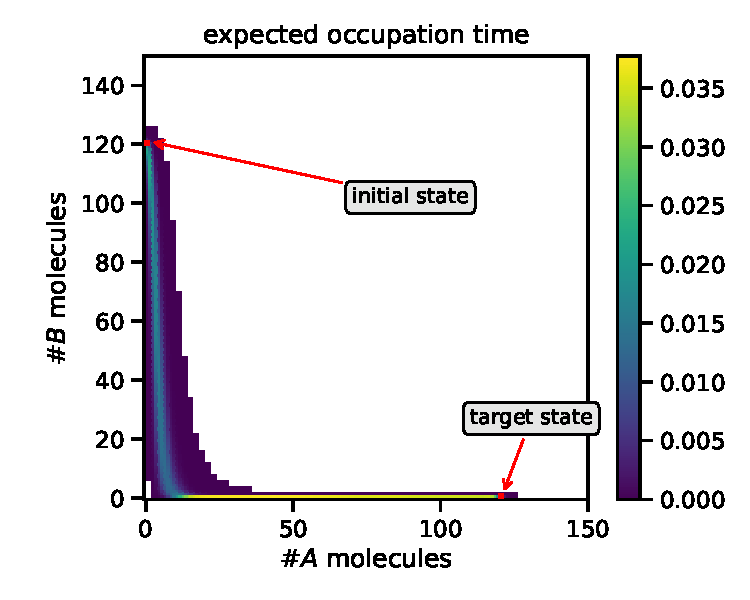
\includegraphics[scale=.6]{gfx/toggle_exp_occ.pdf}
  \caption[Expected occupation time]{The expected occupation time
    (excluding initial and terminal states) for the switching problem
    of the toggle switch using Hill-type functions. The bridging
    problem is from initial $(0,120)$ to a first passage of $(120, 0)$ in
  $t\in [0,10]$.}
  \label{fig:switching_dynamics:occ}
\end{figure}

\subsubsection*{Toggle Switch}
Next, we apply our method to  a toggle switch model exhibiting
non-polynomial rate functions.
This well-known  model considers two proteins $A$ and $B$
inhibiting the production of the respective other
protein~\parencite{lipshtat2006genetic}.
\begin{model}[Toggle Switch using Hill functions]\label{model:hill_toggle}
  We have population types $A$ and $B$ with the following reactions
  and reaction rates.
  $$ \varnothing \xrightarrow{\alpha_1(\cdot)} A\,,\quad
  \text{where}\quad \alpha_1(x) = \frac{\rho}{1 + x_B},
  \qquad A \xrightarrow\lambda \varnothing $$
  $$ \varnothing \xrightarrow{\alpha_1(\cdot)} B\,,\quad
  \text{where}\quad \alpha_1(x) = \frac{\rho}{1 + x_A},
  \qquad B \xrightarrow\lambda \varnothing $$
  The parameterization is $\rho=10$, $\lambda=0.1$.
\end{model}
Due to the non-polynomial rate functions $\alpha_1$ and $\alpha_2$,
the transition rates between macro-states
are approximated by using the continuous integral
\label{page:approx}
\[
  \bar{\alpha}_1(\bar{x})\approx\int_{a-0.5}^{b+0.5} \frac{\rho}{1 +
  x}\, dx = \rho \left(\log{\left(b + 1.5 \right)} - \log{\left(a +
  0.5 \right)} \right)
\]
for a macro-state $\bar{x}= \{a,\dots,b\}$.%\vw{explain $k$ I guess
% it is the mode}%\MB{we don't have mode vars here. it's just $k$ to
% make the expression more clear because then its essentially 1D}

We analyze the switching scenario from $(0, 120)$ to the first visit
of state $(120, 0)$ up to time $T=10$. The initial lumping scheme
covers up to \num{352} molecules of $A$ and $B$ and  macro-states
have size $32\times32$.
The truncation threshold is $\delta=\e{1}{-4}$.
%Transition rates are computed using the above non-polynomial integral.
The resulting truncation is shown in \autoref{fig:switching_dynamics:occ}.
It also illustrates the kind of insights that can be obtained from
the bridging distributions.
For an overview of the switching dynamics, we look at the expected
occupation time under the terminal constraint of having entered state
$(120,0)$. Letting the corresponding hitting time be
\[
  \tau=\inf\{t\geq 0\mid X_t=(120, 0)\}\,,
\]
the expected occupation time for some state $x$ is
\[
  E\left(\int_0^{\tau}1_{=x}(X_t)\,dt\mid \tau\leq 10\right)\,.
\]
We observe that in this example the switching  behavior seems to be
asymmetrical.
The main mass seems to pass through an area where initially a small
number of $A$ molecules is produced followed by a total decay of $B$ molecules.

\subsection{Recursive Bayesian Estimation}
We now turn to the method's application in recursive Bayesian estimation.
This is the problem of estimating the system's
past, present, and future behavior under given observations.
Thus, the \ac{MPM} becomes a \acf{HMM}.
The observations in such models are usually noisy, meaning that we
cannot infer the system state with certainty.

This estimation problem entails more general distributional
constraints on terminal $\beta(\cdot,T)$ and initial $\pi(\cdot, 0)$
distributions than the point mass distributions considered up until now.
We can easily extend the forward and backward probabilities to more
general initial
distributions   and terminal distributions $\beta(T)$.
%This extension is useful for estimating scenarios subject to measurement noise.
For the forward probabilities we get
\begin{equation}
  \pi(x_i, t) = \sum_j \Pr(X_t=x_i\mid X_0=x_j) \pi(x_j,0),
\end{equation}
and similarly the backward probabilities are given by
\begin{equation}
  \beta(x_i, t) = \sum_j\Pr(X_T=x_j\mid X_t = x_i) \beta_T(x_j)\,.
\end{equation}
We apply our method to an \acf{SEIR} model.
This is widely used to describe the spreading of an epidemic such as the current
\acsfont{COVID}-19 outbreak~\parencite{he2020seir,grossmann2020importance}.
Temporal snapshots of the epidemic spread  are mostly only available
for a subset of the population and suffer from   inaccuracies of
diagnostic tests.
Bayesian estimation can then be used to infer the spreading dynamics
given uncertain temporal snapshots.
%Therefore due to the combination of model simulation and the
% uncertain measurements a  problem arises.
%We demonstrate our method on such an estimation problem.
% We assume the full model including parameterization is given.

\begin{model}[Epidemic Spread]\label{model:seir}
  A population of susceptible individuals can contract a disease from
  infected agents. In this case, they are exposed, meaning they will
  become infected but cannot yet infect others. After being infected,
  individuals change to the removed state. The mass-action reactions
  are as follows.
  \[ S + I \xrightarrow{\lambda} E + I\,, \quad
    E \xrightarrow{\mu} I\,, \quad
  I \xrightarrow{\rho} R\,. \]
  The parameter values are $\lambda=0.5$, $\mu=3$, $\rho=3$. Due to
  the stoichiometric invariant $X_t^{(S)} + X_t^{(E)} + X_t^{(I)} +
  X_t^{(R)} = \mathrm{const.}$, we can eliminate $R$ from the system.
\end{model}

We consider the following scenario:
There are $N$ individuals.
We know that initially ($t=0$) one individual is infected and the
rest is susceptible.
At time $t=0.3$ all individuals are tested for the disease.
The test, however, only identifies infected individuals with probability
$p_{\text{tp}}= 0.99$.
Moreover, the probability of a false positive is $p_{\text{fp}} = 0.05$.
\marginpar{The false positive probability is the same for all
non-infected invididuals.}
The random variable $Y_t$ models the measurement likelihood at time $t$.
Based on the description above
\begin{multline*}
  \Pr(Y_t=\hat{n}_I\mid X_t^{(I)} = n_I)\\
  =
  \sum_{k=0}^{\hat{n}_I} B(k; {n_I}, p_{\text{tp}}) B(\hat{n}_I - k ;
  N - n_I, p_{\text{fp}})
  %%%%%%%%\binom{N - n_I}{\hat{n}_I - k}\\
  %%%%%%%%  p_{\text{tp}}^k (1-p_{\text{tp}})^{n_I - k}
  % p_{\text{fp}}^{\hat{n}_I - k} (1 - p_{\text{fp}})^{N - n_I - \hat{n}_I - k}
\end{multline*}
where $B$ is the binomial probability mass function and
\[
  B(k; n, p) = \binom{n}{k}p^k(1 - p)^{n -  k}\,.
\]
We like to identify the distribution given both the initial state and
the measurement at time $t=0.3$.
In particular, we want to infer the distribution over the latent
counts of  $S$ and $E$ by
% The question we like to answer is whether the number of infected
% exceeds the threshold $k=100$ in the time interval $[t,2t]$.
\emph{recursive Bayesian estimation}.

% The first sub-problem is the estimation of the posterior
% distribution at time $t$ given the measurement.
The posterior for $n_I$ infected individuals at time $t$, given
measurement $Y_t=\hat{n}_I$ can be computed using  Bayes' rule
\begin{multline}\label{eq:bayes_posterior}
  \Pr(X_t^{(I)}=n_I\mid Y_t=\hat{n}_I, X_0=x_0)\\ \propto
  \Pr(Y_t=\hat{n}_I\mid X_t^{(I)} = n_I)\Pr(X_t^{(I)}=n_I\mid X_0=x_0)\,.
\end{multline}
This problem is an extension of the bridging problem discussed up until now.
The difference is that the terminal posterior   is   estimated it
using the result of the lumped forward equation and the measurement
distribution using~\eqref{eq:bayes_posterior}.
Based on this estimated terminal posterior, we compute the bridging
probabilities and refine the truncation tailored to the location of
the posterior distribution.
In \autoref{fig:seir:dyn}, we illustrate the bridging distribution
between the terminal posterior and initial distribution.
In the context of filtering problems this is commonly referred to as smoothing.
Using the learned truncation, we can obtain the posterior
distribution for the number of infected individuals at $t=0.3$
(\autoref{fig:seir:t}).
Moreover, can we infer a distribution over the unknown number of
susceptible and exposed individuals (\autoref{fig:latent}).
\begin{figure}[t]
  \myfloatalign
  \subfloat[Prior and posterior dynamics]
  {\label{fig:seir:dyn}
  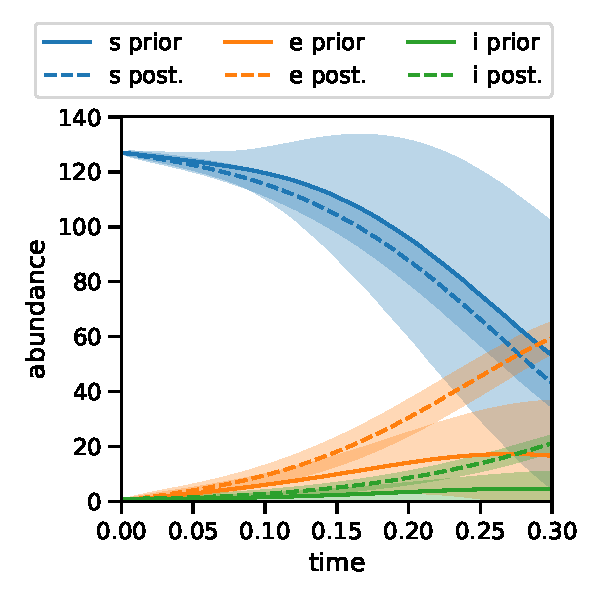
\includegraphics[width=0.48\linewidth]{gfx/seir_prior_posterior.pdf}}
  \subfloat[Beliefs and likelihood at $t=0.3$]
  {\label{fig:seir:t}
  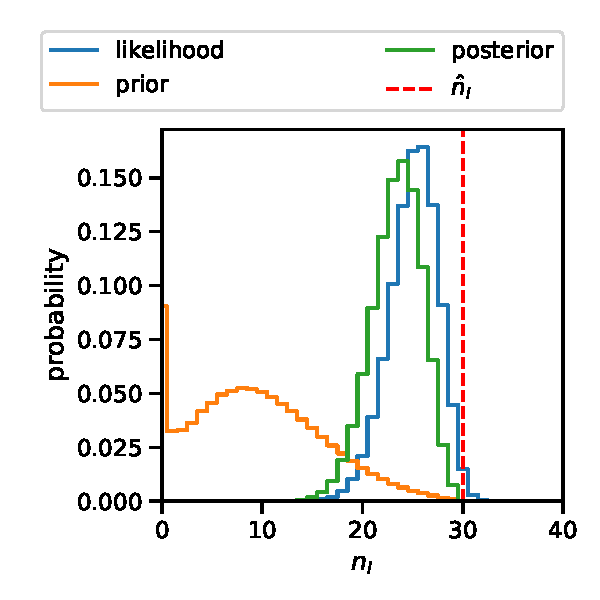
\includegraphics[width=0.48\linewidth]{gfx/posterior.pdf}}
  \caption[Bayesian estimation on the \ac{SEIR} model]{
    (a) A comparison of the prior dynamics and the posterior
    smoothing (bridging) dynamics.
    (b) The prior, likelihood, and posterior of the number of infected
  individuals $n_I$ at time $t=0.3$ given the measurement $\hat{n}_I=30$.}
\end{figure}
\begin{figure}
  \centering
  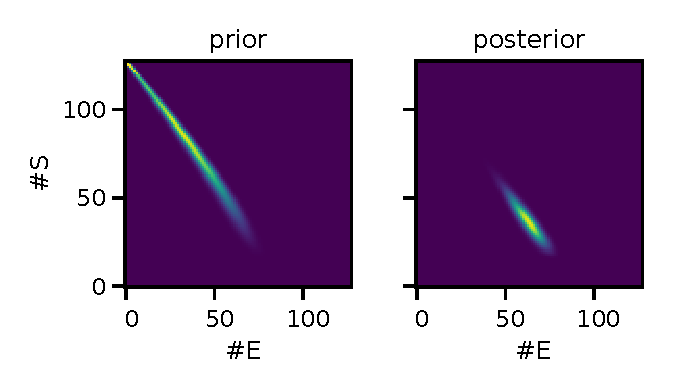
\includegraphics[width=.6\linewidth]{gfx/prior_posterior.pdf}
  \caption[Prior and posterior (\ac{SEIR})]{\label{fig:latent}
    The prior and posterior distribution over the latent types $E$ and
  $S$ at time $t=0.3$.}
\end{figure}

% Using the posterior \eqref{eq:bayes_posterior} of the first
% sub-problem, we can proceed and analyze the bridging problem from
% using the terminal constraint of the infected population exceeding
% threshold $k$.
% To this end this area of the state-space is made absorbing and we
% can proceed as before.
\section{Conclusion}
The analysis of \acp{MPM} with constraints on the initial and
terminal behavior is an important part of many probabilistic
inference tasks such as parameter estimation using Bayesian or
maximum likelihood estimation, inference of latent system behavior,
the estimation of rare event probabilities, and reachability analysis
for the verification of temporal properties.
If endpoint constraints correspond to atypical system behaviors,
standard analysis methods fail
as they have no strategy to identify those parts of the state-space
relevant for meeting the terminal constraint.

Here, we proposed a method that is not based on stochastic sampling
and statistical estimation
but provides a direct numerical approach.
It starts with an abstract lumped model, which is iteratively refined
such that only those parts of the model are considered that contribute to the
probabilities of interest.
In the final step of the iteration, we operate at the granularity of
the original model and compute lower bounds for these bridging
probabilities that are rigorous up to the error of the numerical
integration scheme.
%To achieve accurate bounds, appropriate error tolerances for the
% numerical integration have to be chosen.

Our method exploits the population structure of the model, which is
present in many important application fields of \acp{MPM}.
% As with any direct method based on truncations, our approach is
% limited to models where population sizes remain relatively small.
Based on experience with other work based on truncation, the approach
can be expected to scale up to at least a few million
states~\parencite{mikeev2011efficient}.
Compared to previous work, our method neither relies on
approximations of unknown accuracy nor additional information such as
a suitable change of measure in the case of importance sampling.
It only requires a truncation threshold and an initial choice for the
macro-state sizes.
% Alternatively, uniformization can be applied to strengthen the
% precision guarantees \parencite{mateescu2010fast}.\MB{for backward
% solutions too?; uniformization does not fit with the paragraphs
% opening; schon oben}

In future work, we plan to extend our method to hybrid approaches, in
which a moment representation is employed for large populations while
discrete counts are maintained for small populations.
Moreover, we will apply our method to model checking  where
constraints are described by some temporal logic \parencite{hajnal2019data}.
